\subsection{General Methods}

\begin{theorem}[\textbf{Probability Rules}]
    \phantom{}
    \begin{enumerate}
        \item \textbf{Rule 1:} $P(S) = 1.$
        \begin{proof}
            $\displaystyle P(S) = \sum_{a \in S} P(a) = \sum_{\text{all $a$}} P(a) = 1.$ \\
        \end{proof}
        \item \textbf{Rule 2:} For any event $A$, $0 \leq P(A) \leq 1.$
        \begin{proof}
            $\displaystyle P(A) = \sum_{a \in A} P(a) \leq \sum_{a \in S} P(a) = 1$
            and since each $P(a) \geq 0$, we have $0 \leq P(A) \leq 1.$ \\
        \end{proof}
        \item \textbf{Rule 3:} If $A$ and $B$ are two events with $A \subseteq B$
        (that is, all of the points in $A$ are also in $B$), then $P(A) \leq P(B).$
        \begin{proof}
            $\displaystyle P(A) = \sum_{a \in A} P(a) \leq \sum_{a \in B} P(a) = P(B)$,
            so $P(A) \leq P(B).$
        \end{proof}
    \end{enumerate}
\end{theorem}

\textbf{Venn Diagrams}
% %% This block is what you'll need to put in your code where you want your picture.
% \begin{tikzpicture}
%     %% You can adjust the opacity here. For venn diagrams it is convenient to have a low opacity so that you can see intersections
%         \begin{scope} [fill opacity = .4]
%     %% The draw command knows a lot of shapes. To make a rectangle you just need to specify two diagonal corners. Make sure you always have a semicolon at the end of your draw commands, otherwise latex flips out.
%         \draw (-2,2.5) rectangle (2,-1.3);
%     %% Similarly, you can make a circle by specifying the center and then the radius. You can also add a fill color, but if you're printing in black and white you'll probably want to remove that line.
%         \draw[fill=green, draw = black] (-0.4,1) circle (0.7);
%         \draw[fill=blue, draw = black] (0.4,1) circle (0.7);
%         \draw[fill=red, draw = black] (0,0.3) circle (0.7);
%     %% We can use the node command to label points. If you put your cursor on "LARGE" or "textbf" a box will drop down with size and text style options.
%         \node at (-1.7,2.8) {\LARGE\textbf{S}};
%         \node at (-1,1.8) {\LARGE\textbf{A}};
%         \node at (1.1,1.8) {\LARGE\textbf{B}};
%         \node at (-0.75,-0.4) {\LARGE\textbf{C}};
%         \end{scope}
%     %% And now you have a venn diagram. Yay!
%     %\draw[help lines](-5,5) grid (5,-6);    This line can draw the grid lines to help guide you. I use these when I'm writing the code and then delete this line when I publish the pdf.
% \end{tikzpicture}

% \begin{tikzpicture}
%     \begin{scope} [fill opacity = .4]
%     \draw (8,2.5) rectangle (12,-1.3);
%     \draw[fill=green, draw = black] (9.6,1) circle (0.7);
%     \draw[fill=blue, draw = black] (10.4,1) circle (0.7);
%     \draw[fill=red, draw = black] (10,0.3) circle (0.7);
%     \node at (8.3,2.8) {\LARGE\textbf{S}};
%     \node at (9,1.8) {\LARGE\textbf{A}};
%     \node at (11.1,1.8) {\LARGE\textbf{B}};
%     \node at (9.25,-0.4) {\LARGE\textbf{C}};
%     \end{scope}
% \end{tikzpicture}

\begin{minipage}{0.45\textwidth}
    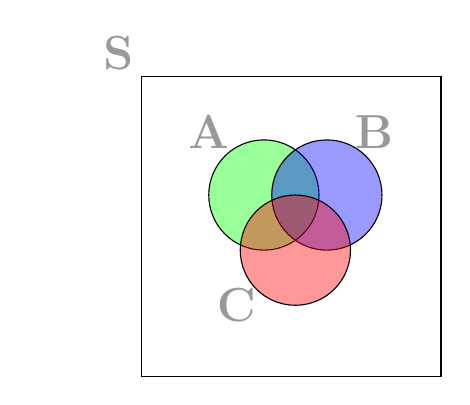
\begin{tikzpicture}
        %% You can adjust the opacity here. For venn diagrams it is convenient to have a low opacity so that you can see intersections
        \begin{scope} [fill opacity = .4]
        %% The draw command knows a lot of shapes. To make a rectangle you just need to specify two diagonal corners. Make sure you always have a semicolon at the end of your draw commands, otherwise latex flips out.
        \draw (0.6,2.5) rectangle (4.4,-1.3);
        %% Similarly, you can make a circle by specifying the center and then the radius. You can also add a fill color, but if you're printing in black and white you'll probably want to remove that line.
        \draw[fill=green, draw = black] (2.15,1) circle (0.7);
        \draw[fill=blue, draw = black] (2.95,1) circle (0.7);
        \draw[fill=red, draw = black] (2.55,0.3) circle (0.7);
        %% We can use the node command to label points. If you put your cursor on "LARGE" or "textbf" a box will drop down with size and text style options.
        \node at (-0.3,2.8) {\LARGE\textbf{\phantom{SB}}};
        \node at (0.3,2.8) {\LARGE\textbf{S}};
        \node at (1.45,1.8) {\LARGE\textbf{A}};
        \node at (3.55,1.8) {\LARGE\textbf{B}};
        \node at (1.8,-0.4) {\LARGE\textbf{C}};
        \end{scope}
        %% And now you have a venn diagram. Yay!
        %\draw[help lines](-5,5) grid (5,-6);    This line can draw the grid lines to help guide you. I use these when I'm writing the code and then delete this line when I publish the pdf.
    \end{tikzpicture}
    \captionof{figure}{$A \cup B \cup C$.}
\end{minipage}%
    \hfill
\begin{minipage}{0.45\textwidth}
    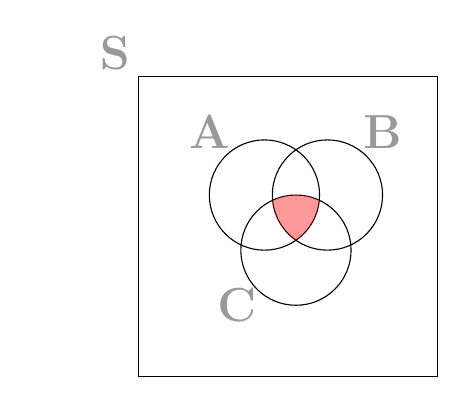
\begin{tikzpicture}
        \begin{scope} [fill opacity = .4]
        \draw (9.4,2.5) rectangle (13.2,-1.3); % add 1.3 to x values
        \draw[fill=none, draw = black] (11,1) circle (0.7);
        \draw[fill=none, draw = black] (11.8,1) circle (0.7);
        \draw[fill=none, draw = black] (11.4,0.3) circle (0.7);

        \begin{scope}
            \clip (11,1) circle (0.7);
            \clip (11.8,1) circle (0.7);
            \fill[red] (11.4,0.3) circle (0.7);
        \end{scope}
        
        \node at (8.3,2.8) {\LARGE\textbf{\phantom{S}}};
        \node at (9.1,2.8) {\LARGE\textbf{S}};
        \node at (10.3,1.8) {\LARGE\textbf{A}};
        \node at (12.5,1.8) {\LARGE\textbf{B}};
        \node at (10.65,-0.4) {\LARGE\textbf{C}};
        \end{scope}
    \end{tikzpicture}
    \captionof{figure}{$A \cap B \cap C$.}
\end{minipage}

\begin{theorem}[\textbf{De Morgan's Laws}]
    \phantom{}
    \begin{enumerate}[label={(\alph*)}]
        \item $\overline{A \cup B} = \overline{A} \cap \overline{B}$
        \item $\overline{A \cap B} = \overline{A} \cup \overline{B}$
    \end{enumerate}
\end{theorem}

\begin{proof}
    \phantom{}  \\
    Use venn diagrams to prove it as an exercise.
\end{proof}




\subsection{Rules for Unions of Events}

\begin{theorem}[\textbf{Rule 4a: Addition Law of Probability or the Sum Rule}]
    \phantom{}  \\
    Let $A$ and $B$ be events (not necessarily mutually exclusive). Then
    \[P(A \cup B) = P(A) +P(B) - P(A \cap B).\]
\end{theorem}

\begin{proof}
    \begin{align*}
        P(A) + P(B) &= \sum_{a \in A} P(a) + \sum_{a \in B} P(a)    \\
                    &= \left(\sum_{a \in A \cap \overline{B} } P(a) + \sum_{a \in A \cap B} P(a)\right)
                       + \left(\sum_{a \in \overline{A} \cap B} P(a) + \sum_{a \in A \cap B} P(a)\right)  \\
                    &= \left(\sum_{a \in A \cap \overline{B}} P(a) + \sum_{a \in A \cap B} P(a)
                             + \sum_{a \in \overline{A} \cap B} P(a)\right) + \sum_{a \in A \cap B} P(a)  \\
                    &= \sum_{a \in A \cup B} P(a) + \sum_{a \in A \cap B} P(a)  \\
                    &= P(A \cup B) + P(A \cap B)
    \end{align*}
    Rearranging the equation, we obtain:
    \[P(A \cup B) = P(A) +P(B) - P(A \cap B),\]
    as desired. This can also be justified by using a Venn diagram. In the expression $P(A) + P(B),$
    the points in $A \cap B$ have their probability counted twice, so they need to be subtracted once.
\end{proof}

\begin{theorem}[\textbf{Rule 4b: Probability of the Union of Three Events}]
    \phantom{}  \\
    Let $A$, $B$ and $C$ be events. then
    \[P(A \cup B \cup C) = P(A) + P(B) + P(C) - P(A \cap B) - P(A \cap C) - P(B \cap C) + P(A \cap B \cap C).\]
\end{theorem}

\begin{proof}
    Use venn diagrams to prove it as an exercise.
\end{proof}

\begin{theorem}[\textbf{Rule 4c: Probability of the Union of $n$ Events}]
    \phantom{}  \\
    A generalization of the above rules to $n$ events $A_1, A_2, \ldots, A_n$. This is often referred to
    as the \textit{inclusion-exclusion principle}.
    \begin{align*}
        P(A_1 \cup A_2 \cup \cdots \cup A_n) = &\sum_{i} P(A_i) - \sum_{i<j} P(A_i \cap A_j)
                                                + \sum_{i<j<k} P(A_i \cap A_j \cap A_k)   \\
                                               &- \sum_{i<j<k<l} P(A_i \cap A_j \cap A_k \cap A_l) + \cdots
    \end{align*}
    (where the subscripts are all distinct).
\end{theorem}

\begin{proof}
    This can be proved using Rule 4a and induction.
\end{proof}

\begin{definition}[\textbf{Mutually Exclusive}]
    Events $A$ and $B$ are \textbf{mutually exclusive} if \[A \cap B = \emptyset.\]
\end{definition}

\begin{remark}
    We can extend this definition to events $A_1, A_2, \ldots, A_n$.
\end{remark}

\begin{example}
    If a die is rolled twice, the events $A = \text{ "2 occurs on the 1st roll"}$ and
    $B = \text{ "total is 10"}$ are mutually exclusive events.
\end{example}

\begin{theorem}[\textbf{Rule 5a: Probability of the Union of Two Mutually Exclusive Events}]
    \phantom{}  \\
    Let $A$ and $B$ be mutually exclusive events. then
    \[P(A \cup B) = P(A) + P(B).\]
\end{theorem}

\begin{theorem}[\textbf{Rule 5b: Probability of the Union of $n$ Mutually Exclusive Events}]
    \phantom{}  \\
    In general, let $A_1, A_2, \ldots, A_n$ be mutually exclusive events. then
    \[P(A_1 \cup A_2 \cup \cdots \cup A_n) = \sum_{i=1}^{n}P(A_i).\]
\end{theorem}

\begin{proof}
    This can be proved from Rule 5a using induction or as an immediate consequence of Rule 4c.
\end{proof}

\begin{theorem}[\textbf{Probability of the Complement of an Event}]
    \phantom{}  \\
    For any event $A$, we have \[P(A) = 1 - P(\overline{A}).\]
\end{theorem}

\begin{proof}
    $A$ and $\overline{A}$ are mutually exclusive and $A \cup \overline{A} = S$, so by Rule 5a,
    \begin{align*}
        P(A \cup \overline{A}) &= P(A) + P(\overline{A})    \\
                             1 &= P(A) + P(\overline{A})    \qquad \left( \text{since $P(A \cup \overline{A}) = 1$} \right)    \\
                 \implies P(A) &= 1 - P(\overline{A}).
    \end{align*}
\end{proof}

\begin{example}
    Two fair dice are rolled. Find the probability that at least one of them turns up a six. \\
    \textbf{Solution 1: } Defining appropriate events: \\
    $A = \left\{  \text{outcome from first die is a 6} \right\}$ and $B = \left\{  \text{outcome from second die is a 6} \right\}$.
    Therefore, either first is a 6 and second is a six OR both give a 6. \\
    $\implies P(A \cup B) = P(A) + P(B) - P(A \cap B) = \frac{1}{6} + \frac{1}{6} - \frac{1 \times 1}{36} = \frac{11}{36}$.

    \textbf{Solution 2:} Using the complement: \\
    $\implies P(\text{at least one 6}) = 1 - P(\text{zero 6s}) = 1 - \frac{5 \times 5}{36} = \frac{11}{36}$.
\end{example}


\subsection{Intersections of Events and Independence}

\begin{definition}[\textbf{Independent and Dependent Events}]
    Events $A$ and $B$ are \textbf{independent events} $\iff P(A \cap B) = P(A)P(B).$
    Otherwise, we call the events \textbf{dependent}.
\end{definition}

Independence means that knowing information about $A$ will not affect the information about $B$.

\begin{definition}
    The events $A_1, A_2, \ldots A_n$ are mutually independent if and only if
    \[P(A_{i_1} \cap A_{i_2} \cap \cdots \cap A_{i_k}) = P(A_{i_1}) P(A_{i_2}) \cdots P(A_{i_k})\]
    for all sets $(i_1, i_2, \ldots, i_k)$ of distinct subscripts chosen $(1, 2, \ldots, n)$.
\end{definition}



\subsection{Conditional Probability}

\begin{definition}[\textbf{Conditional Probability}]
    \phantom{}\\
    The \textbf{conditional probability} of event $A$, given event $B$, is
    \[P(A | B) = \frac{P(A \cap B)}{P(B)}, \quad \text{provided $P(B) > 0.$}\]
\end{definition}

\begin{note}
    $P(A|B) = 1 - P(\overline{A}|B)$.
\end{note}

\begin{theorem}
    \phantom{}  \\
    Suppose $A$ and $B$ are two events defined on a sample space $S$ \st $P(A) > 0$
    and $P(B) > 0.$ Then $A$ and $B$ are independent events $\iff$ either of the following
    statements is true;
    \[P(A|B) = P(A) \quad \text{OR} \quad P(B|A) = P(B).\]
\end{theorem}

\begin{example}[\textbf{exercise}]
    You ask your roommate to water a sickly plant while you are on vacation. Without water, the plant will die with probability 0.8 and with water
    it will die with probability 0.1. Your roommate will remember to water the plant with probability 0.85. \\
    If the plant is alive when you return, what is the probability that your roommate remembered to water it? \\
    \textbf{Answer: } The probability is 0.9623. \\
\end{example}

\begin{example}[\textbf{exercise}]
    The probability a randomly selected male is colour blind is 0.05, whereas the probability a female is colour blind is 0.0025. If the population is
    50\% male, what fraction of the population is colour blind? \\
    \textbf{Answer: } The probability is 0.02625.
\end{example}

\newpage


\subsection{Product Rules, Law of Total Probability and Bayes' Theorem}

\begin{theorem}[\textbf{Rule 7: Product Rules}]
    \phantom{}  \\
    Let $A, B, C, D, \ldots$ be arbitrary events in a sample space. Assume that $P(A) > 0$,
    $P(A \cap B) > 0$, and $P(A \cap B \cap C) > 0$. Then
    \begin{align*}
        P(A \cap B) &= P(A)P(B|A)     \\
        P(A \cap B \cap C) &= P(A)P(B|A)P(C|A\cap B)     \\
        P(A \cap B \cap C \cap D) &= P(A)P(B|A)P(C|A\cap B)P(D|A\cap B\cap C)    \\
        &\vdots
    \end{align*}
\end{theorem}

\begin{proof}
    Use the definition of the conditional probability $P(B|A)$.
\end{proof}

\begin{note}
    Used when finding intersections given conditional probabilities.
\end{note}

\begin{theorem}[\textbf{Rule 8: Law of Total Probability}]
    \phantom{}  \\
    Let $A_1, A_2, \ldots, A_k$ be a partition of the sample space $S$ into disjoint
    (mutually exclusive) events, that is 
    \[A_1 \cup A_2 \cup \cdots \cup A_k = S \quad \text{and} \quad A_i \cap A_j = \emptyset \quad \text{if $i \neq j$.}\]
    Let $B$ be an arbitrary event in $S$. Then
    \begin{align*}
        P(B) &= P(B\cap A_1) + P(B\cap A_2) + \cdots + P(B\cap A_k)    \\
             &= \sum_{i=1}^{k} P(B|A_i) P(A_i).
    \end{align*}
\end{theorem}

\begin{example}[\textbf{exercise}]
    At a police spot check, 10\% of cars stopped have defective headlights and a faulty muffler. 15\% have defective headlights and a
    muffler which is satisfactory. If a car which is stopped has defective headlights, what is the probability that the muffler is also faulty? \\
    \textbf{Answer: } The probability is 0.4.
\end{example}

\pagebreak


\begin{theorem}[\textbf{Bayes' Theorem}]
    \phantom{}  \\
    Suppose $A$ and $B$ are events defined on a sample space $S$. Suppose also that
    $P(B)  > 0$. then
    \[P(A|B) = \frac{P(B|A) P(A)}{P(B)} = \frac{P(B|A) P(A)}{P(B|\overline{A}) P(\overline{A}) + P(B|A) P(A)}.\]
\end{theorem}

\begin{proof}
    \begin{align*}
        \frac{P(B|A) P(A)}{P(B|\overline{A}) P(\overline{A}) + P(B|A) P(A)} &=
        \frac{P(A \cap B)}{P(B \cap \overline{A}) + P(B \cap A)}  \qquad \text{by the Product Rule}   \\
        &= \frac{P(A \cap B)}{P(B)}   \qquad \text{by the Law of Total Probability}  \\
        &= P(A|B).
    \end{align*}
\end{proof}

\begin{remark}
    Bayes' Theorem applies when given "opposite conditions", i.e. we want to find $A|B$ given $B|A$.
\end{remark}



\newpage